% COLONNA SINGOLA E AUTORE-DATA, non IEEEtran a due colonne.
% La destinazione e' EMSE. `registro/EMENDAMENTO-07` aveva posto una condizione invece di una
% preferenza: «non si converte al template Springer prima di sapere se la prima sottomissione lo
% richiede... da verificare sulle istruzioni per autori prima di spendere lavoro di
% impaginazione». La verifica non era mai stata fatta, e un seggio di presentazione ha segnalato
% che la prima cosa che ogni pagina dice a un editor e' il formato sbagliato.
% Verificato il 19/08: il template Springer NON e' obbligatorio alla prima tornata, ma lo stile
% dei riferimenti e' autore-data e l'impaginazione e' a colonna singola (le figure si preparano
% per un'area di testo a colonna singola da 174 mm). Quindi si converte il formato, non il
% template: `article` a colonna singola con `natbib`/`plainnat`, che soddisfa entrambe le
% convenzioni senza dipendere da un file di classe che non ho.
\documentclass[11pt,a4paper]{article}
\usepackage[margin=2.6cm]{geometry}
\usepackage[round]{natbib}

\usepackage{amsmath}
\usepackage{amssymb}
\usepackage{booktabs}
\usepackage{graphicx}
\graphicspath{{figures/}}
\usepackage{xcolor}
\usepackage[hidelinks]{hyperref}

% L'UNICO punto in cui inserire il link al deposito anonimo. Il paper dichiara che
% l'artefatto e' citato nella sottomissione, e quella frase e' vera solo se qui c'e' un
% URL. Finche' e' vuoto, la macro stampa un segnaposto ben visibile e la build RIFIUTA di
% produrre l'archivio: e' l'unico modo per non spedire per distrazione una promessa non
% mantenuta, che in C1 il pannello di riproducibilita' ha classificato come fatale.
% `xurl` al posto di `url`: in colonna singola l'URL del deposito sbordava di 80,9pt perche'
% `url` non spezza dentro un percorso. `xurl` lo spezza dove capita, che per un URL e' corretto.
\usepackage{xurl}
\newcommand{\artifacturl}{\url{https://github.com/<utente>/transport-endpoint-agentic-eval}}
% Il repository e' il deposito operativo; il DOI permanente si ottiene all'accettazione,
% ed e' l'unico modo di ottenerlo. La sezione Data Availability dichiara entrambe le cose
% invece di promettere un DOI come se esistesse.

\begin{document}

% Ordine di lettura. Il censimento dei meccanismi di cancellazione sta DOPO i risultati e
% PRIMA della discussione: riporta sull'apparato che ha prodotto i numeri appena dati, e
% le sue voci si leggono solo una volta che i risultati le hanno rese concrete.
% La formula viene dal capitolo precedente del programma, che e' sotto revisione anonima: titolo e
% sede non si nominano nemmeno qui, perche' i commenti viaggiano col sorgente e il sorgente E' il
% deposito. Il commento che stava qui dichiarava questa regola e poi citava quel titolo per esteso
% due righe sotto -- la stessa forma del documento di redazione che annullava la redazione che
% dichiarava. Rimosso il 19/08. La struttura che si eredita e' descrivibile senza nominare nulla:
% prima meta' parallela, due punti, poi cosa viene comprato e a spese di cosa. La serie si
% riconosce a colpo d'occhio, e chi legge un capitolo solo non perde niente.
%
% Il titolo nomina MECCANISMI, non una magnitudine: nessun test supera la propria soglia di
% Holm, e annunciare "il trasporto cambia le prestazioni" sarebbe marketing nei numeri invece
% che nella formulazione.
%
% Il sottotitolo porta entrambe le gambe, e non sono in parallelo. Quanto del punteggio compra
% l'interfaccia e' un BIAS, si delimita, e dopo BFCL non e' piu' una notizia. Quali modelli
% l'endpoint toglie prima che tu misuri e' una SELEZIONE, non si delimita perche' il modello
% assente non ha una riga da correggere, e li' cade il peso probatorio.
% L'ordine delle due gambe segue quello dei contributi, che il 16/08 e' stato invertito: la
% SELEZIONE viene prima del BIAS, perche' un bias si delimita e una selezione no. Il titolo
% precedente prometteva per primo cio' che il paper ora dichiara secondo.
% TITOLO — descrittivo, non a slogan. La formula del capitolo precedente
% Free Parameter: …») e' da conferenza; i titoli EMSE dicono cosa e' stato fatto: «An evaluation
% study of…», «Reflections on the Reproducibility of…», «Empirical benchmarking of…». Un editor
% deve poterlo classificare al primo sguardo, e «pre-registered» in prima pagina e' un segnale
% che quella sede legge. La serie con il capitolo precedente resta visibile dal contenuto e
% dalla citazione, che e' dove serve.
\title{Transport and Endpoint as Free Parameters in Agentic Evaluation:\\
\large A Pre-Registered Study of Four Models Across Two Clouds}

% EMSE fa revisione a CIECO SINGOLO (verificato sulle politiche del journal, 2026-08-15):
% autore e affiliazione vanno dichiarati. Un blocco anonimo qui sarebbe un difetto per questa
% destinazione, non una precauzione.
%
% Affiliazione verificata online il 2026-08-15: dottorato in ICT presso il DISIM, che ospita il
% programma (phdict.disim.univaq.it), e la dicitura estesa del dipartimento e' quella usata
% dalle pubblicazioni dell'ateneo.
%
% Autore unico, per decisione dell'autore. Il lavoro precedente (EASE 2025, «Simplicity by
% Obfuscation») e' firmato De Tomasi, Di Sipio, Di Marco, Nguyen; questo capitolo no, e le
% dichiarazioni finali sono al singolare di conseguenza.
% Il dominio e' graduate.univaq.it, quello dei dottorandi, non student.univaq.it che Scholar
% riporta: corretto dall'autore.
\author{<autore>\\[0.4em]
\normalsize Department of Information Engineering, Computer Science and Mathematics (DISIM)\\
\normalsize University of L'Aquila, L'Aquila, Italy\\
\normalsize \texttt{lorenzo.detomasi@graduate.univaq.it}}
\date{}

\maketitle

\begin{abstract}
An agentic evaluation reports a number for a model, but that number is produced by an apparatus --- a
transport carrying tool calls, an endpoint serving them --- named in no table. We measure how much of it
belongs to the apparatus: four models, two managed clouds (Databricks and Amazon Bedrock), two transports,
45 held-out reverse-engineering tasks, 5,809 trials, analysis script frozen by hash with the hypotheses
before any data existed (two of the ten tests were implemented a day later under a dated succession, when
the data on disk could not inform either --- \S\ref{sec:method}).

Three results, in the order a reader should weigh them: two exploratory, one confirmatory. First, the
variance components of an agentic measurement are specific to the apparatus that produced them, and that
breaks study sizing. Inheriting a calibration from an earlier chapter on the same corpus, model and
metric, ours did not mis-estimate a magnitude --- it inverted which lever binds: 84\% run-to-run noise
and a floor of thirteen tasks became 0.5\% (bootstrap interval $[0.0, 1.4]$ over 45 binaries) and a floor
of 668. A designer who inherited it would not merely have been under-powered; they would have spent the
budget on the axis that buys nothing.

Second, an endpoint can remove a model from an evaluation entirely, and we document \emph{eight}
mechanisms across eleven probed models, each with the endpoint's verbatim message. Six are reachable by a
pre-flight probe --- protocol refusal, deprecation, absent quota, disuse, jurisdiction, parallel calls ---
and two fire only in a conversational state a probe does not construct, so a harness certified healthy
before collection can still lose a cell after the money is spent. This is a selection effect rather than
a bias: the refused model has no row to correct. Removing one model from a four-model comparison moves
the first-to-last spread by up to 47.6pp, against 9.83pp for the largest apparatus effect we measure.

Third, the confirmatory family resolves no effect at the available precision --- none of the ten tests
survives correction, and the three reaching nominal significance are the three least powered (21.0\%,
30.9\%, 35.8\%). That is not a finding of no effect. We report the minimum detectable effect per contrast
rather than one figure for the design, because the observed standard deviations span a factor of 23.7:
resolving power is a property of the cell, not of the study.
\end{abstract}

% EMSE chiede da 4 a 6 keywords: erano sette. Tolta «reproducibility», che e' implicata da
% pre-registration ed experimental validity insieme.
\vspace{0.6em}
\noindent
\textbf{Keywords} agentic evaluation $\cdot$ tool calling $\cdot$ experimental validity $\cdot$
pre-registration $\cdot$ serving infrastructure $\cdot$ selection effects

% RICHIESTO DALLA LETTERA DI RITORNO (EMSE-D-26-00987): il numero di trial clinico va sulla
% title page, e se non si applica va scritto che non si applica. La richiesta viene dal
% flusso editoriale Springer condiviso con le riviste biomediche; qui non si applica, e
% dichiararlo costa una riga mentre ometterlo e' costato una restituzione.
\vspace{0.5em}
\noindent
\textbf{Clinical trial number:} not applicable.

\section{Introduction}
\label{sec:intro}

An agentic evaluation reports a number for a model. That number is produced by an apparatus:
a transport that carries tool calls between the model and the harness, an endpoint that serves
the weights, a set of tools with a particular return format, and a decoding configuration. The
model's name appears in the table. The apparatus does not.

This paper measures how much of that number the apparatus determines rather than the model, and finds
two answers of different kinds. The transport moves a number, which is a
bias. The endpoint deletes a row, which is a selection. A bias can be bounded, and a reader who knows
its size can correct for it. A selection cannot, because the model that was
refused has no line in the table to correct.

\subsection{The confound this study removes}

A companion study~\citep{companion2026baseline} measured a 10.4pp drop when one model moved from native
function calling to a textual protocol. It is a companion manuscript
under double-anonymous review, so a reader cannot obtain it. Both figures this paper draws from it
recompute from a snapshot of the exact cells they need, released in the deposit with their per-turn logs. On a single infrastructure that number admits two readings no
further collection on that infrastructure can separate --- a property of the model, or of that
provider's shim --- because model and infrastructure are perfectly confounded when there is only one
endpoint.

Serving the same nominal model from two managed clouds tests something a single endpoint cannot: whether
the measured outcome changes across deployed services at fixed nominal model identity. It does not, by
itself, say which component of a service produced any difference it finds --- the two stacks differ in
several observable quantities at once (\S\ref{sec:runtime}) --- but a difference that survives the change
of service is a difference the model's name alone does not describe. That cell --- same nominal model, two
commercial endpoints, transport manipulated as a paired factor, on a multi-turn downstream task --- is what
this study contributes as a design, and to our knowledge it has not been run.

\subsection{Contributions}

The order below is the one in which we would have a reader weigh them, not the one in which they were
planned. \textbf{The first is the primary contribution: it does not rest on a $p$-value, and it is
checkable by re-issuing the probes we release.}

\begin{enumerate}
\item \textbf{Eight mechanisms by which a serving endpoint removes a model from an evaluation before it
  produces a score, or destroys its measurements from inside one}, each with the endpoint's message
  (\S\ref{sec:census}). They fall into four operational classes --- lifecycle and access policy,
  capability and API-contract constraint, catalogue and quota inconsistency, integration and adapter
  incompatibility --- and they sit at three levels of detection difficulty, which is the operational
  finding: four are returned to an ordinary single-request capability check, three need a deliberately
  constructed conversational state, and one appears only when the model itself emits the output that
  triggers it. For the three that a single-request check does not reach we give the constructed probe that
  does, and for the last we give the trajectories in which it fired.
\item \textbf{Temperature zero is not determinism}, measured across the corpus: one model returns
  identical runs on 91--100\% of binaries and another on 20--24\% (\S\ref{sec:results}). That output
  distributions can differ between services at fixed model identity is already
  established~\citep{gao2025equality}; in one of eight comparisons here the difference reaches the
  \emph{stability of a downstream agentic score}, which is the extension this study contributes on that
  axis.
\item \textbf{A pre-registered $4\times2\times2$ design} --- four models, two named managed clouds, two
  transports, 45 held-out binaries, 8 runs each --- with the analysis script frozen by hash
  \emph{together with} the hypotheses before collection began; two of the ten tests were implemented
  under a timestamped amendment after it had (\S\ref{sec:method}). No test passes its Holm threshold.
  We report per contrast the effect its own observed dispersion would have let it resolve, because those
  dispersions span a factor of 23.7 and no single band describes them.
\item \textbf{A variance calibration that inverts on its own data.} This design was sized expecting
  run-to-run noise to dominate; measured here, the lever that binds is the number of tasks --- 0.5\% noise
  and a floor of 668 binaries on the contrast with the largest observed dispersion
  (\S\ref{sec:rq6}). Whether such
  calibrations transfer between apparatuses is a question this raises and does not settle, and the stronger
  reading is a proposition rather than a result (\S\ref{sec:proposizioni}).
\item \textbf{An artifact} carrying every raw row including the invalidated batches, the per-turn session
  traces, the frozen documents with their hashes, and the amendment log (\S\ref{sec:artifact}).
\end{enumerate}

\subsection{The boundary of the claim}

Three boundaries fix what follows. The transport contrast measures that the choice moves the number, not
which choice is right. The eight mechanisms are existence proofs, each with its own denominator rather than
a rate, and the class is open by construction. And the effect sizes belong to the scope
\S\ref{sec:threats} bounds.

\textbf{The transferable output of this study is the checklist of Table~\ref{tab:checklist} and the
variance-decomposition method, not the coefficients.} Two of the four models are open-weight, so the task,
the corpus and the harness can be re-run on infrastructure a reader controls --- though not this design:
every cell here was served by one of the two commercial clouds, and a self-hosted re-run would be a
different apparatus, which is precisely the property under study. The propositions of
\S\ref{sec:proposizioni} are hypotheses this study instantiates, not claims it establishes. The narrower
claim made here is that an evaluation which does not report its transport is not reproducible from its
method section, whatever the task.
\section{Related Work}
\label{sec:related}

This section positions the work against its neighbours and states the delta at the width the evidence
supports.

\subsection{Measurement bias, and the harness as its current object}

The shape of our finding is old in systems research and new only in the evaluation of agents: that a
measurement depends on the stack under it is unremarkable in performance work, where declaring the
configuration is a norm. What agentic evaluation lacks is that norm. The argument has been made for the
harness as a whole~\citep{zhang2026harness,yao2026harnessbench}; this study is downstream of it and supplies the
measurement it lacks --- what the undeclared choices are worth, one axis at a time.

Four lines of work bound this one, and the artifact expands each with the figures we take from it.
\textbf{Apparatus variance is established methodology elsewhere}: rigorous performance measurement has
long required reporting the configuration and treating run-to-run variation as first
class~\citep{georges2007rigorous,iosup2011variability}, and measurement bias from unreported setup
choices was demonstrated two decades ago~\citep{mytkowicz2009wrongdata} --- what is missing here is not
the method but its application. \textbf{Non-determinism at nominal temperature zero} has been measured for repeated
sampling~\citep{atil-nondeterminism} and traced to the batch size a server happens to be
running~\citep{he2025nondeterminism} --- the class of server-side quantity our \S\ref{sec:runtime} finds
differing between two services at fixed model identity. \textbf{The endpoint is already known to be a service rather than an artifact}: a measurement study of
hosted open-weight APIs finds one model differing across providers in protocol support, error semantics,
context capacity and throughput~\citep{li2026service}, which is our T5--T8 axis arrived at independently.
\textbf{And the transport axis is visible to the field, in no fixed direction}: a leaderboard ranks every
model in a native and a prompted mode~\citep{bfcl2025}; on one model the prompted variant is \emph{ahead}
by 6pp~\citep{bfcl-leaderboard,bfcl-issue606}; on an agentic tool-use benchmark a prompt-based protocol
severely degrades a model of the same family as our T3/T4, attributed to a template mismatch with the
model's training~\citep{mcpverse2025}; and a third transport, tools as typed code stubs rather than JSON,
matches or exceeds native calling on 11 of 14 models~\citep{bitterlesson2026}. Three transports, and no
direction that survives a change of task family --- which is what makes the axis a parameter to declare
rather than a correction to apply. \textbf{And the task family has its own literature}:
reconstruction from stripped binaries is active~\citep{tan2024llm4decompile,jiang2025nova}, semantic
equivalence under LLM-driven transformation has been evaluated directly, on a different corpus and
task~\citep{detomasi2025obfuscation}, test-based equivalence has known
limits~\citep{liu-wang-issta2020}, and the reproducibility of published results built on
commercial models has been assessed directly, with model deprecation as a leading cause of
failure~\citep{angermeir2026reproducibility}.

\subsection{The transport: known to move the number, in no fixed direction}

The nearest thing to a counterexample is the leaderboard above: it ranks every model in both a native and a
prompted mode, so the axis is not invisible to the field. It reports the two modes side by side rather than
crossing them with the serving endpoint, and on one model the prompted variant is \emph{ahead} by
6pp~\citep{bfcl-leaderboard,bfcl-issue606} --- which we treat as a constraint on our claim rather than as
support. Designing on an effect size estimated from earlier data is known to miss its target
power~\citep{albers2018power}; what this case adds is a direction that reverses rather than drifts.

The reporting obligation is already established and we do not argue for it: community guidelines for
empirical work with language models require the harness to be described when it goes beyond bare API
calls~\citep{baltes2026guidelines}. Those guidelines do not make all of the apparatus fields examined here
equally explicit, and Table~\ref{tab:checklist} says which. What this study supplies is the other half: how much the
choices in question move a measured number.

\subsection{The endpoint: a unit of measurement, and a unit of selection}

\textbf{That two services can serve one model identity and return different output distributions is
established, and measured at scale.} A two-sample test on the Maximum Mean Discrepancy, applied to
commercial inference APIs for four Llama models, finds \textbf{11 of 31 endpoints serving distributions
that differ from the reference weights} --- naming Amazon Bedrock and Azure AI Studio among the access
paths, at a median 77.4\% power against a range of distortions~\citep{gao2025equality}. That work settles
the premise this study starts from, and it does so on raw output distributions from single prompts: it
crosses no transport, runs no multi-turn agentic task, and says nothing about whether the divergence
reaches a downstream score. What \S\ref{sec:results} adds is one case where it reaches the
\emph{stability} of such a score.

Holding weights, decoding and hardware fixed while varying only the inference engine produces measurable
differences in output, which establishes the mechanism this study extends: if an engine moves a number at fixed
weights, a managed platform choosing engine, version and scaffolding without disclosing any of them can
move it too, and a reader has no way to know by how much~\citep{silent-hyperparameter}.

Removal also breaks reproduction downstream, and its scale has been measured on one public arena's
own roster: of 243 models, 205 had been silently deprecated against 47 marked as such, at rates of
87.8\% for open-weight and 80\% for proprietary models~\citep{leaderboard-illusion}. That audit
names the mechanism --- ``Chatbot Arena may be forced to deprecate a model when a provider no longer
supports it via its API'' --- and counts the outcome after the fact, aggregated over a roster; this census measures the refusals themselves, verbatim and case by case, before a score exists.

\subsection{What the census adds to the failure taxonomies}

The nearest neighbour to our census is a taxonomy of failure modes in multi-provider serving
infrastructure, classified by origin layer and detectability~\citep{failureatlas}. Two of its
five layers already reach failures occurring before generation --- network and transport covers
``TCP timeouts, TLS handshake failures, DNS resolution issues'', governance and cost covers
``rate-limit counters that leak and never recover'' --- so the distinction we draw is not about
\emph{when} the failure lands.

What the census adds is a different question, asked one step earlier: not how a request fails once a
model is being served, but \emph{whether this endpoint will serve this model identity at all}, under this
request contract, from this account and this region. Several of our mechanisms are access and lifecycle
decisions rather than defects, and those persist for the duration of a study whoever is judged
responsible; others --- the request-contract constraints and the adapter incompatibility --- could
reasonably be filed as bugs by an operator who owns them. \textbf{Nothing in our contribution depends on
which filing a reader prefers}: what \S\ref{sec:tassonomia} establishes is that mechanisms of this class
exist, where in the evaluation lifecycle they act, what they cost a measurement, and that they need
different detection. The artifact carries the layer-by-layer comparison for a reader who wants to place
each row.


\section{Method}
\label{sec:method}

\subsection{The task}

Each trial gives a model one stripped x86-64 binary, decompiled with a static analysis server, and asks
it to reconstruct compilable C source. The candidate is compiled in a pinned container and executed
against the unit tests of the original program, and the score is the fraction that pass.

Pass-rate is a \emph{lower bound} on semantic equivalence and we report it as such throughout: a
candidate correct but differing in an untested behaviour scores below one, and one wrong in an untested
behaviour scores above its true worth. We use it because it is executable and adversarially hard to game,
not because it is tight.

\subsection{Pre-registration}

The hypotheses, the test family, the falsifiers, and \emph{the analysis script} were frozen by
content hash before a single row of data existed. Registered reports have been available in this
field since 2020~\citep{ernst2023registered}; what we add is the second half of that freeze.

Two of the ten tests are an exception we state here rather than let a reader find it in the artifact,
because the exception is the more informative case. T9 (heterogeneity across models) and T10
(transport $\times$ infrastructure interaction) were declared in the family at the freeze but emitted a
non-computable $p$, and were implemented eleven hours later under a dated succession document written
\emph{before} the change. Collection had begun, so the freeze does not cover them strictly, and their
guarantee is a weaker but checkable property: neither could be informed by the data that existed ---
three cells were on disk, all of a \emph{single} model, while T9 compares the transport effect
\emph{between} models and T10 needs both transports on both infrastructures, one of which had not
started. Both entered Holm at the $m=10$ fixed before any data existed, so the correction they face was
not chosen after seeing them. Fixing the hypotheses while writing the analysis after seeing the data
leaves intact every degree of freedom pre-registration exists to remove: which test, on which subset,
with which exclusion. Every subsequent change to a frozen file is documented before the change and
checked by a guard, and the register is in the artifact.

\subsection{The two transports}

The manipulated variable is how a tool call travels between the model and the harness. Both
transports offer the same tools, the same schemas, and the same twelve turns.

\textbf{Native.} The request carries a \texttt{tools} field. The model emits a structured
tool-call object, which the runtime parses; results return in the role the provider's API
defines for tool output.

\textbf{Textual.} The request carries \emph{no} \texttt{tools} field. The system prompt
defines a line protocol: the model ends its reply with a single line
\texttt{TOOL\_CALL:}~followed by a JSON object naming the tool and its arguments. The
harness parses that line and returns the result as an ordinary user message.

Two consequences bound what the contrast means, and both belong before any number. First, the native
transport admits more than one call per turn where the text protocol admits one by construction.

\begin{table}[h]
\caption{Batching under the native transport, per model. The text protocol is fixed at one
call per turn by construction, so the confound is present only where this rate exceeds one.}
\label{tab:batching-rate}
\centering
\small
\begin{tabular}{lrrl}
\toprule
model & calls/turn & turns $>1$ & contrast affected \\
\midrule
haiku & 1.438 & 38\% & T3 \\
sonnet & 1.333 & 33\% & T4 \\
gpt-oss & 1.000 & 0\% & --- \\
llama & 1.000 & 0\% & --- \\
\bottomrule
\end{tabular}
\end{table}

The confound is structurally available to every model and binds only where the model uses it, which
two of four do not at all. Second, \emph{a turn that produces prose without a tool call is not a
failure}: it is a turn without a call and is recorded as such, since treating it as a terminal answer
would end the trajectory at turn one and score the protocol rather than the model.

\subsection{What counts as a measurement}

One predicate decides whether a row is a measurement, and collector and analysis use the same one --- two
definitions of validity, one per half of a pipeline, diverge silently. It has two clauses, and we state
them here because every number in this paper is computed over the rows they admit: a row is a measurement
unless the endpoint reported an infrastructure failure, or the harness itself raised. Rows the predicate
rejects are kept in the released data with the reason attached --- they are the subject of
\S\ref{sec:census}, not attrition --- and the artifact states the failure that motivated each clause.



\section{Experimental Design}
\label{sec:design}

\subsection{Research questions}
\label{sec:rqs}

Six questions organise what follows: three answered by the pre-registered family, three by evidence
labelled exploratory wherever it appears. They expound a design frozen before collection --- no
hypothesis, test or comparison is added, and the family stays at $m=10$ (\S\ref{sec:family}).

\begin{table}[t]
\centering
\caption{The six questions, what answers each, and its status. Confirmatory items map onto
hypotheses frozen before collection; exploratory items are reported as such throughout.}
\label{tab:rqs}
\small
\begin{tabular}{@{}p{0.07\linewidth}p{0.55\linewidth}p{0.30\linewidth}@{}}
\toprule
 & question & answered by \\
\midrule
RQ1 & By how much does the transport of a tool call move the measured score, at fixed model
      and infrastructure? & H1, tests T1--T4 \emph{(confirmatory)} \\
RQ2 & By how much does the serving endpoint move it, at fixed model and transport? &
      H2, tests T5--T8 \emph{(confirmatory)} \\
RQ3 & Is the transport's effect constant across models, and do transport and endpoint
      interact? & H3 and H4, tests T9--T10 \emph{(confirmatory)} \\
RQ4 & By which mechanisms does an endpoint remove a model from an evaluation before it
      produces a score? & the census, \S\ref{sec:census} \emph{(exploratory)} \\
RQ5 & How much of the transport difference is the loss of call batching rather than the
      change of format? & the constrained-native arm, \S\ref{sec:rq5}
      \emph{(exploratory)} \\
RQ6 & Does a power calibration transfer between apparatuses that share model, corpus and
      metric? & \S\ref{sec:results} \emph{(exploratory)} \\
\bottomrule
\end{tabular}
\end{table}

RQ4 through RQ6 were not all asked at the outset: RQ4 was pre-registered as an exploratory census,
while RQ5 and RQ6 are questions the apparatus raised while it ran. What protects them is not that they
were anticipated but that each is answered by a quantity a reader can recompute --- verbatim endpoint
responses, an arm with a stopping criterion fixed in advance, and two calibrations from two
apparatuses.

\subsection{The grid}

Four models, each served by both Databricks and Amazon Bedrock under two transports: sixteen cells. We
name the platforms rather than abstract them --- the venue is single-blind, and the mechanisms of
\S\ref{sec:census} quote the endpoints verbatim, so a reader recognises the platform from the message
whatever we call it and can re-issue each probe against the platform that produced it. Every cell runs
the same 45 held-out binaries eight times, so the design plans 5{,}760 trials while the primary
re-collection delivers 5{,}809 and the replication batch 5{,}805. The three numbers differ for one
reason: a run returning an infrastructure failure is logged as a record and \emph{re-run}, so a cell can
end with more valid measurements than the 360 it planned. The surplus --- 49 above plan and 45 --- is not
a bonus but the count of runs an endpoint refused or dropped, which \S\ref{sec:census} treats as the
subject rather than as attrition, and one cell ends \emph{below} plan at 44 binaries of 45 for the reason
given in \S\ref{sec:ottavo}. Turn budget, temperature and output cap are identical in every cell and
recorded per row rather than assumed.

\begin{table}[h]
\caption{The grid. Every cell is the same corpus under a different apparatus.}
\label{tab:grid}
\centering
\small
\begin{tabular}{ll}
\toprule
models & 4 (two open-weight, two proprietary) \\
infrastructures & 2 (Databricks, Amazon Bedrock) \\
transports & 2 (native, textual) \\
cells & $4\times2\times2 = 16$ \\
binaries per cell & 45, held out, frozen by hash \\
runs per binary & 8 \\
trials & 5{,}760 planned, 5{,}809 measured \\
turn budget & 12 \\
temperature & 0.0 \\
\bottomrule
\end{tabular}
\end{table}

\subsection{Why we say \emph{nominal} model}

Throughout we write \emph{nominal model} rather than \emph{the same weights}. Two managed
clouds advertising the same open-weights model may serve different quantisations, different
runtime versions, or route to a different variant under load, and neither exposes enough to
settle it. Verifying byte-identity is not possible from the outside, so we do not claim it: what
we hold fixed is the model \emph{identity a user selects}, which is exactly the thing a
published evaluation names in its table.

This is not a hedge, it is the object of study. If two endpoints selling the same name behave
differently, that difference belongs in the method section of every paper that names the model
and not the endpoint --- whether the cause is the weights, the runtime, or the routing.

\subsection{Hypotheses, and why two of them are disjunctive}

We ask whether the transport moves the score at fixed infrastructure (H1), whether the
infrastructure moves it at fixed transport (H2), whether the transport's effect is constant
across models (H3), and whether transport and infrastructure interact (H4).

This matters for how the result is read. An interval that excludes effects above some
magnitude is not the same claim as no difference, and we never write the second when the data
support only the first.

\subsection{The test family, and why its size does not shrink}
\label{sec:family}

Ten tests were pre-registered as one family with Holm step-down. The family size is fixed. It
does not shrink when a cell turns out to be inconclusive, uninteresting, or unexecutable,
because removing a member after seeing the data lowers the thresholds of every survivor --- a
correction that grows more permissive exactly as one learns which tests one would like to
pass.

One consequence is deliberate and worth naming: the family includes contrasts nobody
disputes, and those contrasts consume correction budget. That is the price of fixing $m$
before the data exist, and it is cheaper than the alternative.

\subsection{Six defaults inherited from the preceding chapter}

Six constraints are inherited from the preceding chapter, each traceable to a defect that produced a
clean and false number: unwrapped candidate source, functions in native order, symbol tables stripped,
a reasoning-only turn not recorded as a zero, a price guard that refuses \emph{before} the provider
call, and the token-limit parameter sent under the one name the endpoint accepts. None is a discovery
--- each is a default a competent implementer would set, which is what makes the list worth publishing
--- and the artifact states each with the defect it answers.

% L'ORDINE E' DELIBERATO, e segue quello delle Contributions in §I invece di contraddirlo.
% Il censimento viene prima dei contrasti perche' e' il risultato che non dipende da un p-value:
% un endpoint ha restituito quel messaggio o non l'ha fatto. Nella versione precedente il lettore
% incontrava dieci test che non superano la correzione PRIMA della parte che regge, e l'elenco dei
% contributi diceva l'opposto dell'ordine in cui il corpo li presentava.
\section{RQ4 \emph{(pre-registered as exploratory)}: What the Endpoint Removes Before a
Score Exists}
\label{sec:census}

\textbf{Eight of the 21 model-platform pairs we attempted never produced a score; five of the 18 on the
two platforms the design measures.} The third platform is Azure, probed while assembling the sample and
then left out of the arms. This is the result that does not depend on a $p$-value --- an endpoint either
returned the message we quote or it did not --- and it is reported at a scale a reader can size.

\textbf{Three quantities are counted here, each in its own unit and with its own denominator.}
\emph{(A)} Pairs removed before measurement: 8 of 21 attempted, spanning
11 distinct models, traceable to 7 distinct causes --- six of them are the mechanisms M1--M6 below and the
seventh is a reasoning-channel case the deposit carries. \emph{(B)} Losses inside a cell that had already
started: M7 cost 453 rows of one cell, discarded and re-collected; M8 rejected 11 trajectories across the
two retained collections --- four in the original collection of 5{,}805 valid measurements, seven in the
re-collection of 5{,}809. \emph{(C)} Distinct mechanisms
documented: 8, of which 6 act before a score exists and 2 from inside a run. \textbf{Each is an existence
proof with its own denominator, and no incidence rate over models or platforms is computed from them.}

\textbf{The removals are not distributed evenly across the three platforms, and both denominators are
therefore reported.} Databricks 2 removals of 8 pairs attempted, Bedrock 3 of 10, \textbf{Azure 3 of 3}: the
overall 8 of 21 becomes 5 of 18 on the two measured platforms, 27.8\% against 38.1\%, a difference of 10.3
points resting on three attempts against one infrastructure. Three mechanisms below were observed only
there, which is why Table~\ref{tab:mechanisms} names the platform for each. Azure stays in the denominator
because dropping it would report a smaller number by discarding the attempts that failed most, and both
fractions are properties of an assembled roster rather than of managed clouds
(\S\ref{sec:proposizioni}).

Building the sample required probing which models each infrastructure would serve, and that probe returned
six mechanisms. Two more appeared from inside the confirmatory arm, where the roster probe does not reach
them: eight in total, none sought.

\subsection{The eight mechanisms, with the endpoint's own words}

\textbf{Every row is bounded to the configuration that produced it}, listed per mechanism in the deposit:
one endpoint, one API surface, one region, one set of parameters. The wording throughout is that the service
rejected the request under the evaluated configuration, not that the platform does not support the
feature. Where
variants were tried --- two identifier forms on M4, three history shapes on M6, the three admissible
tool-choice values on M7 --- the deposit records them, and those three rows can be stated more sharply for
that reason.

\begin{table}[!t]
\caption{The eight mechanisms, each an existence proof with its own denominator rather than a rate.
\textbf{Class} is operational and says what kind of thing the removal is, which is what decides who can do
anything about it: \emph{lifecycle} is an access or retirement policy, \emph{contract} is a constraint of
the API's own request contract, \emph{quota} is an inconsistency between what a catalogue advertises and
what the quota system holds, \emph{adapter} is an incompatibility between the format a model emits and the
validation the serving layer applies to it. \textbf{Scope} says how far the decision reaches:
\emph{vendor} holds for everyone on that platform, \emph{region} depends on where the request originates,
\emph{tenant} depends on the account's own history and quota, so two teams on one platform see different
rosters. \textbf{Det.} is the probe that reaches the mechanism, from the matrix in the deposit:
\emph{1} an ordinary single-request capability check, \emph{2} a deliberately constructed conversational
state, \emph{3} detectable only when the model itself emits the triggering output. Quoted cells are the
endpoint's words under the evaluated configuration, truncated to one line; M3 is a three-step control-plane
observation and is set unquoted for that reason. The deposit carries every message in full with the request
and the configuration that produced it.}
\label{tab:mechanisms}
\centering
\small
\setlength{\tabcolsep}{3pt}
\begin{tabular}{@{}l P{0.155\linewidth} l l l c P{0.375\linewidth}@{}}
\toprule
& mechanism & platform & class & scope & det. & verbatim message \\
\midrule
M1 & protocol refusal & Databricks & contract & vendor & 2 & \texttt{400}: multi-turn tool calls unsupported \\
M2 & deprecation & Azure & lifecycle & vendor & 1 & \texttt{ServiceModelDeprecated \ldots\ since 06/13/2026} \\
M3 & absent quota & Azure & quota & tenant & 1 & catalogue advertises it, quota system has no row, creation refused \\
M4 & disuse & Bedrock & lifecycle & tenant & 1 & \emph{``marked by provider as Legacy and you have not been actively using the model''} \\
M5 & jurisdiction & Bedrock & lifecycle & region & 1 & \emph{``Access to Meta Llama models is not allowed from unsupported countries''} \\
M6 & parallel calls & Azure & contract & vendor & 2 & \texttt{400 UnsupportedToolUse}: \emph{``does not support more than one tool call''} \\
M7 & tool config not expressible & Bedrock & contract & vendor & 2 & tool-choice admits ``auto'', ``any'', a named tool --- not ``none'' \\
M8 & endpoint rejects its own model's output & Bedrock & adapter & vendor & 3 & \texttt{ValidationException}: tool name fails \texttt{[a-zA-Z0-9\_-]+} \\
\bottomrule
\end{tabular}

\vspace{0.3em}
{\footnotesize Detection level 2 means a probe exists and must be built: for M1 a history already carrying
one tool call and its result; for M6 a history carrying two calls inside a single assistant message; for M7
a history carrying a tool-use block in a request that offers no tools. Each is one request once assembled.
Level 3 admits no such probe: the request must carry a tool name the model itself generated.}
\end{table}

Table~\ref{tab:mechanisms} is not a taxonomy derived from documentation: every row is a message an endpoint
returned to a request we made. M1--M6 were found by probing which models each infrastructure would serve;
M7 and M8 appeared from inside the confirmatory arm.

\textbf{The detection column is the operational finding, and it is a gradient rather than a split.} Four
mechanisms answer a single ordinary request. Three --- M1, M6 and M7 --- are invisible to any check that
sends one call per turn, and become one request each only once the conversational state is assembled by
hand; a harness certified healthy by an ordinary capability check can therefore still lose a cell after the
money is spent. M8 admits no probe at all in this sense, because what triggers it is generated by the model
during the run. The practical consequence for a pre-flight is that it must exercise realistic
conversational states, and that even then one class of failure remains reachable only by collecting.

For M6 the three-request sequence below separates the levels directly, and M7 is defined by a request
shape only a history containing a tool call can produce; M1's reproducer is the agentic exchange its
message names.

\subsection{Commentary on M6, M7 and M8}

\textbf{On M6.} The state it needs --- a history in which the model has already emitted two calls inside
one assistant message --- is one no single request constructs, but it \emph{is} constructible, and
assembling it by hand turns the mechanism into a probe answerable before any collection is paid for. Its
verification was three requests: one tool at turn one passes, a history with one prior tool call passes, a
history with two calls in one assistant message is refused.

\textbf{On M7.} The protocol we pre-registered ends each trajectory with a turn that offers no tools, and
under the evaluated Bedrock Converse configuration that turn \emph{cannot be expressed}: the API requires a
tool configuration whenever the history contains a tool call, and its tool-choice parameter admits
``auto'', ``any'' and a named tool --- but not ``none''. We tried the three admissible values and omitting
the configuration entirely; none expresses the turn.

\textbf{M7 is the easiest of the three level-2 mechanisms to have found, and we did not find it that
way.} The constraint is in the vendor's public API reference, which documents the tool-choice parameter as
a union of exactly three members with no value for ``no tools'': it was knowable before this study existed,
by reading, without issuing a request. M1 and M6 have no such public statement that we could locate, and
were reached by probing. The operative lesson is therefore not that M7 was undiscoverable but that
\emph{nobody checked the pre-registered protocol's termination shape against the target API's documented
request contract} --- a check that costs one page of reading and would have saved a 453-row cell.

The exposure was not where it first appeared. The broken rows carried an infrastructure-failure flag and
were already excluded from every mean; what survived was structural. A trajectory reaches the final turn
with a tool call in its history only if it has \emph{not} already submitted through a tool, so the runs
that completed were exactly those that had submitted early --- a second selection effect, inside the axis
this study exists to measure cleanly. That batch of 453 rows was discarded and the cell re-collected against
a corrected client. M7 sits at the same detection level as M6 and for the same reason: an ordinary
capability check reports it healthy, because it fires only in a conversational state that check does not
assemble.

\textbf{On M8.}
\label{sec:ottavo}
The open-weights model emits tool calls in its own chat format, which uses special tokens to separate
reasoning channels. The serving layer does not strip that token from the tool name, so the name reaches the
API as \texttt{decompile\_function<|channel|>commentary}. The API then validates the name it was just
handed:

\begin{quote}\footnotesize\ttfamily\raggedright
ValidationException: Value at\\
'messages.10.member.content.1.member.toolUse.name'\\
failed to satisfy constraint: Member must satisfy\\
regular expression pattern: [a-zA-Z0-9\_-]+
\end{quote}

\noindent
and rejects the entire request --- not the turn, the trajectory. \textbf{That sequence is what is reported here:
a name generated by the served model reaches the same service's request validation and is rejected there.}
It occurred in 11 trajectories, four in the original collection and seven in the re-collection, all in the
one cell where that model meets that endpoint under the native transport. Retrying does not reliably
recover the run: on one binary the cell logged 15 attempts for 7 valid measurements, one of the eight
rejected attempts carrying this exception verbatim and the other seven recording no candidate. Nothing in
the released evidence identifies where in the stack the format a model emits and the validation of the
service's own API fail to meet, and it is not assigned here.

Four further observations belong to the census and not to a paper of this length, and the deposit carries
each with its verbatim evidence. One carries an obligation that transfers: under a service control policy
that permits invocation while denying enumeration, the roster cannot be recovered from the account and must
be declared by explicit enumeration, which is what \S\ref{sec:design} does.

\subsection{How far a removal moves a published comparison}
\label{sec:bound}

That a refused model has no row to correct does not by itself say how much a reader's conclusion changes.
The census documents real cases --- a Llama variant deprecated on one platform while another serves it, a
second blocked by jurisdiction while its siblings run --- so someone evaluating on one endpoint reads a
table with rows missing and does not know which. We bound the consequence on the four models scored on both
clouds, removing one at a time and recomputing the comparison the way a leaderboard reports it. The
\emph{order} survives: all pairwise orderings agree before and after every removal. The \emph{scale} does
not, and with four models its collapse is close to arithmetic --- removing the lowest scorer necessarily
compresses a first-to-last spread --- so what these data support is the sign and the order of magnitude
rather than a coefficient. The artifact carries the eight removals with their per-cloud figures.

\subsection{What the census adds to what is already catalogued}
\label{sec:tassonomia}

The closest neighbour is a taxonomy of failure modes in multi-provider serving, classified by origin layer
and detectability~\citep{failureatlas}. What this census adds does not depend on where any single row is
filed in it, and that independence is deliberate: a reader who prefers to call M3 a configuration bug and
M8 an integration bug can do so, and four things stand unchanged.

\begin{enumerate}
\item \textbf{Multiple distinct removal mechanisms exist and were met in one small study} --- eight, none
  sought, each with the verbatim response of the endpoint that produced it.
\item \textbf{They sit at different points of the evaluation lifecycle.} Six act before any score exists,
  so the experimental unit is missing rather than mismeasured; two act inside a run that had already been
  paid for.
\item \textbf{Their measurement consequence is structural.} A removed pair has no row to correct, which is
  a selection and not a bias, and \S\ref{sec:bound} bounds what that does to a published comparison.
\item \textbf{They require different detection.} Four answer an ordinary capability check, three require a
  constructed conversational state, and one is reachable only during execution --- so a pre-flight that
  sends one request per model does not cover the class.
\end{enumerate}

\noindent
The question none of the existing layers asks is the one that decides whether a model appears in a
benchmark at all --- \emph{will this endpoint serve this model identity, under this request contract, from
this account and this region?} That is a reporting obligation before it is a taxonomic one, and it is where
Table~\ref{tab:checklist} puts it. There is no claim that nobody has catalogued serving failures; the artifact
carries the layer-by-layer comparison so a reader can place each row wherever they judge it belongs.

\section{Analysis and Interpretation}
\label{sec:results}

The census establishes that an endpoint can remove a model before a score exists. This section asks
how far the surviving numbers move, and answers with the resolving power attached.

All numbers here come from the re-collection: an independent execution of the full
$4\times2\times2$ design on workspaces isolated per cell, comprising 5{,}809 valid measurements.
That this batch, rather than the original one, would carry the primary analysis was fixed in
writing before it produced a row (\S\ref{sec:threats}); the original collection is reported
alongside it as a replication, and the two agree on every criterion declared in advance.

% L'ORDINE DELLE SOTTOSEZIONI E' DELIBERATO. La decomposizione della varianza e l'inversione
% della calibrazione vengono prima della famiglia confermatoria: sono il risultato che regge, e
% mettere dieci test che non superano la correzione davanti a essi faceva arrivare il lettore alla
% parte debole per prima.
\subsection{Which lever binds is a property of the cell}
\label{sec:varianza}

The variance of a paired difference decomposes into within-binary noise, which shrinks with more runs
per binary, and heterogeneity between binaries, which shrinks only with more binaries. The two are not
interchangeable, and Table~\ref{tab:variance} shows the choice is not a property of the axis.

% Generata da analysis/tabella_principale.py --varianza su results/riraccolta.
\begin{table}[t]
\caption{Variance decomposition. $K_\infty$ is the number of binaries needed to resolve 3pp with unlimited runs per binary. $\dagger$: on these two contrasts the components are \textbf{poorly identified at the boundary} --- the estimated noise exceeds the observed variance, and the bootstrap clamps the residual to zero in 86\% of replications on T7 and 69\% on T8. No component is reported for them, in either direction: a clamped estimate is a boundary artefact, and printing a precise zero would report the constraint rather than the data. T1, T3 and T6 clamp in at most 1\% of replications, and are the rows the decomposition is read on.}
\label{tab:variance}
\centering
\small
\begin{tabular}{llrrr}
\toprule
& axis & SD & \% noise & $K_\infty$ \\
\midrule
T3 & transport & 0.2774 & 0.5\% & 668 \\
T6 & endpoint & 0.2189 & 9.1\% & 380 \\
T4 & transport & 0.1409 & 20.6\% & 137 \\
T1 & transport & 0.2002 & 46.1\% & 189 \\
T2 & transport & 0.0916 & 61.0\% & 28 \\
T5 & endpoint & 0.1292 & 93.1\% & 10 \\
T7 & endpoint & 0.0117 & \multicolumn{2}{c}{not decomposable$^\dagger$} \\
T8 & endpoint & 0.0585 & \multicolumn{2}{c}{not decomposable$^\dagger$} \\
\bottomrule
\end{tabular}
\end{table}


For T3 and T6 more runs buy nothing: 668 and 380 binaries against the 45 collected.

\textbf{These are estimates on 45 units, so we report their intervals.} Bootstrapping the binaries ---
the unit the contrast is paired on, 5{,}000 replications at a declared seed --- gives T3's noise share
as 0.5\% $[0.0, 1.4]$ and $K_\infty$ as 668 $[265, 1136]$, and T6's as 9.1\% $[4.1, 21.6]$ and 380
$[126, 744]$. The interval on $K_\infty$ is wide and its lower end is still six times the 45 binaries
collected, which is the operational point: the conclusion that more runs buy nothing does not depend on
the point estimate. Neither interval reaches the 50\% that would make the noise share
indistinguishable from half.

\textbf{Where the estimator is misspecified, we say so rather than offer two readings.} The rows marked
$\dagger$ have estimated noise exceeding the observed variance --- not a finding about those cells but a
variance model that does not fit them, since the decomposition assumes the two conditions' runs are
independent given the binary and clamps the residual at zero when that fails. The bootstrap makes the
failure countable: the residual is clamped in \textbf{86\%} of replications on T7, 69\% on T8 and 43\%
on T5, so for those contrasts the lower bound of $K_\infty$ is zero by construction rather than by
evidence, and we report no decomposition for T7 and T8. On T1, T3 and T6 --- the contrasts that carry
the finding --- clamping occurs in at most 1\% of replications.

\subsubsection*{What the metric's granularity does and does not explain}
\label{sec:granularita}

A decomposition of variance is only as trustworthy as the measurement it decomposes, and ours is coarse:
pass-rate over five unit tests gives a run \emph{six} values, 53\% of the 5{,}809 rows sit at an extreme and
33\% of the 720 binary-by-cell means land exactly on 0 or 1. A floor- and ceiling-heavy measurement is on its
own sufficient for a large between-binary spread, so it is a rival account of Table~\ref{tab:variance} and
not only of the inversion that follows.

\textbf{Two conditions bound the account, and both are stated so that a reader can check them.} It would
have to explain why the same metric on the same corpus yields 0.5\% noise here and 84\% in the collection
this design inherited its sizing from --- granularity is a property of the metric, and a property the two
share cannot by itself produce a difference between them. The second condition is narrower than the first and we state it as such: resampling binaries bounds the
sampling variance of the estimate, not a measurement bias, so the interval $[0.0, 1.4]$ on T3 does not by
itself exclude a floor-and-ceiling pattern uniform across the corpus --- such a pattern would reproduce in
every resample. The first condition carries the argument on its own, and neither is closed by these data
alone.

The operational consequence is in \S\ref{sec:proposizioni}: a design resting on a variance
decomposition should size the number of tests per task the way it sizes the number of tasks, and
report the share of runs at floor and ceiling beside the decomposition. We did the second and not
the first.

What T3 and T6 share is not the axis but the pairing of largest observed standard deviation with
smallest nominal $p$: where the effect looks largest it also varies most between binaries, which is
a weaker claim than a large average effect.

\subsection{RQ6 \emph{(exploratory, arose during execution)}: the power calibration
inherited from the previous chapter inverted}
\label{sec:rq6}

The pre-registration states, from the previous chapter's data, that for haiku ``84\% is
run-to-run noise and the floor is $K=13$''. On the same nominal contrast here, the noise share
is $0.5\%$ and the floor is $K=668$.

This is a reversed mechanism rather than a magnitude error, and it survives three independent changes:
of estimator, which widens it to 130.7\% noise and $K=0$; of apparatus and workspace isolation, where the
two collections give 0.1\%/705 and 0.5\%/668; and the other high-variance contrast, 9.3\%/487 against
9.1\%/380. The artifact carries each recomputation.

\textbf{The 84\% comes from the batch in which a validity flag failed, and the three robustness checks above
do not touch that.} Crashed rows were averaged as zeroes there (\S\ref{sec:method}), and the released
snapshot lets a reader reconstruct both computations. We claim no direction for that defect: independent
reconstructions disagree, and on that corpus the corrected estimator is misspecified in the sense of
\S\ref{sec:varianza}, so the quantity one would compare against is clamped rather than estimated. What the
reconstruction does establish is that the inherited 84\% is the \emph{defective} computation, which is why
the inversion is not read off the comparison: it is established inside this chapter by two collections of
our own, 0.1\%/705 and 0.5\%/668 on the contrast that carries it.

One caveat is removed by none of the three: the chapters differ in apparatus as well as estimator, and
exposure to the largest information leak of \S\ref{sec:threats} was asymmetric between arms in the earlier
chapter --- 100\% of native runs invoked the affected tool against 86.7\% of textual runs --- so the
comparison does not isolate the estimator. The inversion is larger than 13pp of differential exposure
makes plausible as a sole cause, but that is an order-of-magnitude argument, not an exclusion. What does
not depend on the comparison is this chapter's own decomposition: the 0.5\% noise share and the
668-binary floor are computed on our data alone and under one estimator, so the finding that the binding
lever is a property of the apparatus stands whether or not the earlier number is right.

\subsection{RQ1--RQ3 \emph{(confirmatory)}: a negative registered result, and the resolving
power that is the reportable quantity}

This subsection reports a \emph{negative} pre-registered result and reports it as such: hypotheses,
test family and analysis were fixed before the data existed, the family does not resolve an effect, and
the outcome is stated before the exploratory findings that did produce something. What it contributes
is not the absence of an effect but the \emph{resolution} at which the absence was established, which
differs by a factor of 23.7 between contrasts sharing one design.

Of the ten tests fixed in the pre-registration, \emph{none} passes its Holm threshold at
$m=10$~\citep{holm1979}. The smallest $p$ is $0.0191$ against a threshold of $0.0050$. No contrast places its
effect outside the $\pm 3$pp falsifier band with a confidence interval that excludes it.

\textbf{Part of that null follows from the family's fixed composition.} Two of the ten tests are not
independent of the other eight, so Holm at $m=10$ divides the smallest threshold by ten rather than
eight --- $0.0050$ instead of $0.0063$. T6's $p$ of $0.0191$ misses both, so no conclusion turns on the
choice here, though on a study whose smallest $p$ fell between them it would; we keep $m=10$ because the
pre-registration fixed it and because it is the conservative direction, not as the only defensible
count. The artifact carries both series.

That answers RQ1--RQ3 in the direction of ``not at this resolution'', and the resolution is the
reportable quantity: an evaluation that cannot separate 4pp from zero is not free to call two transports
equivalent. The outcome does not rest on the $t$'s normality assumption either ---
Appendix~\ref{sec:appendice-permutazione} repeats the family under a distribution-free sign-flip test and
no test passes Holm there.

We report the family outcome together with the achieved power, never one without the other, because
the three contrasts with nominal $p<0.05$ are also the three least powered --- and reporting power at
all is the exception here: 103 software engineering experiments were found systematically below
accepted norms~\citep{dyba2006power}, a decade after the concern was raised as ``missing and
misunderstood''~\citep{miller1997power}, and documented again for language-model
evaluation~\citep{card2020power}.

% Generata da analysis/tabella_principale.py su results/riraccolta — non modificare a mano.
\begin{table}[t]
\caption{The ten pre-registered tests, on the re-collection (isolated workspaces). $\delta$ is the paired difference per binary, over 45 binaries of 8 runs each. \textbf{Sign convention}: for transport contrasts $\delta = \text{textual} - \text{native}$, so a negative value means the textual protocol scores lower; for endpoint contrasts $\delta = \text{Bedrock} - \text{Databricks}$. MDE is the effect this contrast could have resolved at 80\% power given its own observed standard deviation, in percentage points --- the column exists because it varies by a factor of 23.7 across contrasts of one design. Power is computed against the pre-registered MDE of 4.87pp using the \emph{observed} standard deviation and the non-central $t$ --- the distribution the test actually uses. A normal approximation would report 0.0--1.9 points higher, which in a paper reporting its own under-powering would err in the flattering direction. $^\ddagger$The $p$ column is the \emph{exact} Student series, not the approximation the frozen script emits: the approximation understates $p$ in eight cases of eight --- for T6, 0.0155 against 0.0191 --- always in the direction that makes an effect look more significant. Both series are in the artifact, the distribution-free series is in Appendix~\ref{sec:appendice-permutazione}, and no test passes its Holm threshold under any of the three. $^{\P}$T5 is the one contrast whose $p$ rests on $K{=}44$ while its $\delta$ and interval rest on $K{=}45$: one binary returned seven valid runs of eight on one endpoint, the frozen script averages it and the exact-$p$ script requires a full complement. We print both rather than harmonise them, because harmonising would mean choosing a rule after seeing what it does to a pre-registered number.}
\label{tab:tests}
\centering
\scriptsize
\setlength{\tabcolsep}{2.2pt}
\begin{tabular}{llrrrrr}
\toprule
& contrast & $\delta$ & 95\% CI & $p$$^\ddagger$ & power & MDE \\
\midrule
T6 & llama,\, endp. & $-7.94$ & $[-14.5,-1.4]$ & 0.0191 & 30.9\% & 9.14 \\
T3 & haiku,\, transp. & $-9.83$ & $[-18.2,-1.5]$ & 0.0218 & 21.0\% & 11.59 \\
T1 & gpt-oss,\, transp. & $-6.56$ & $[-12.6,-0.5]$ & 0.0334 & 35.8\% & 8.36 \\
T9 & heterogeneity & --- & --- & 0.1011 & --- & --- \\
T2 & llama,\, transp. & $+2.22$ & $[-0.5,+5.0]$ & 0.1107 & 93.7\% & 3.82 \\
T5$^{\P}$ & gpt-oss,\, endp. & $+3.26$ & $[-0.6,+7.1]$ & 0.1159 & 69.6\% & 5.40 \\
T7 & haiku,\, endp. & $+0.22$ & $[-0.1,+0.6]$ & 0.2095 & 100.0\% & 0.49 \\
T8 & sonnet,\, endp. & $-0.94$ & $[-2.7,+0.8]$ & 0.2844 & 100.0\% & 2.44 \\
T10 & interaction & $-4.12$ & $[-10.6,+2.3]^{\S}$ & 0.3448 & --- & --- \\
T4 & sonnet,\, transp. & $-1.00$ & $[-5.2,+3.2]$ & 0.6363 & 62.1\% & 5.88 \\
\bottomrule
\end{tabular}
\end{table}


\begin{figure}[t]
\centering
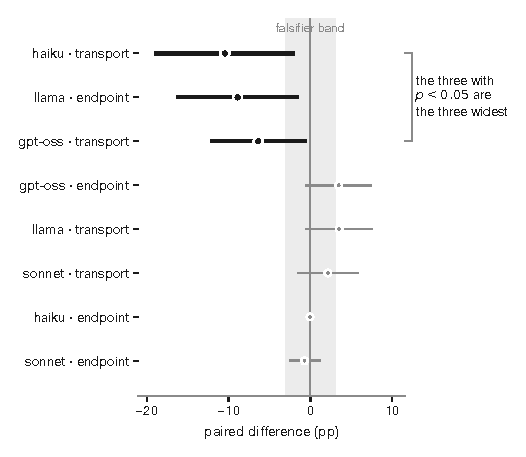
\includegraphics[width=0.78\textwidth]{fig1-effetti-potenza.pdf}
\caption{The ten contrasts, ordered by nominal $p$. Filled and heavier lines are the three
with $p<0.05$ uncorrected; none survives Holm correction. They are also the three widest
intervals in the study --- the signature of a winner's curse, not of a larger effect. Dotted
lines mark the pre-registered $\pm3$pp falsifier band.}
\label{fig:effects}
\end{figure}

Table~\ref{tab:tests} and Fig.~\ref{fig:effects} are the whole confirmatory result. T3 reproduces the
transport difference that motivated this chapter at $-9.83$pp --- different apparatus, isolated
workspaces, three information leaks closed (\S\ref{sec:threats}) --- and T6 shows $7.94$pp between two
clouds serving the same nominal model at fixed transport. Neither survives correction for multiplicity,
and both sit below a third of the power the design was sized for. All three are true together.

$^{\S}$ The frozen script prints no interval for T10; this one is computed outside it with the \emph{model}
as the unit of replication ($n=4$, $t_3$). Treating the 180 binary-level pairs as independent would give a
narrower interval and a wrong one: they are four groups of 45.

\subsection{RQ1--RQ3 \emph{(confirmatory)}: the resolving power is per contrast, not a
single band}

The pre-registration sized the design with a pooled standard deviation of $0.1062$ and a
conservative $0.1167$, both calibrated on the previous chapter. The observed standard
deviations of the paired differences span $0.0117$ to $0.2774$ --- a ratio of 23.7 --- so a
single minimum detectable effect describes the design rather than the data. Computed per
contrast, the MDE ranges from $0.49$pp (haiku across endpoints) to $11.59$pp (haiku across
transports), and \emph{five of eight contrasts exceed} the 4.87pp the design assumed.

A null result here therefore reads: no contrast places its effect outside the band its own variance
permits. It does \emph{not} read as equivalence --- $K=45$ does not power an equivalence test at 3pp,
which would need 99--119 binaries, and this was declared before the data existed.

\subsection{RQ5 \emph{(exploratory, arose during execution)}: evidence against call
batching as the explanation}
\label{sec:rq5}

The pre-registered transport contrast moves two things at once on the models that batch: the format of
the call and the number a turn admits --- haiku issues 1.438 calls per turn against sonnet's 1.333. A
declared confound is not a bounded one, so we collected the arm that separates them: native transport
forced to \emph{one call per turn}, all else held fixed. It is exploratory, does not enter the family of
ten, and its stopping criterion was fixed before it ran.

\begin{table}[t]
\centering
\caption{Constraining the native transport to one call per turn. Paired on binaries, $K=45$,
eight runs per binary. The arm is exploratory and does not enter the corrected family.}
\label{tab:batching}
\footnotesize
\setlength{\tabcolsep}{4pt}
\begin{tabular}{@{}lrrrc@{}}
\toprule
model & full & constr. & diff. & 95\% CI \\
\midrule
haiku-4-5 & 0.747 & 0.754 & $+0.8$pp & $[-2.6, +4.2]$ \\
sonnet-4-5 & 0.793 & 0.809 & $+1.6$pp & $[-1.3, +4.4]$ \\
\bottomrule
\end{tabular}
\end{table}

Removing batching does not lower the score: both differences are \emph{positive} and both intervals
contain zero (Table~\ref{tab:batching}), against a transport effect of $-9.83$pp on the same model and
endpoint. The direction is what the arm supports --- a mechanism cannot explain a decrease it does not
produce --- and that inference needs only the sign of the two differences, which is why it survives the
arm's missed validity band (\S\ref{sec:rq5b}): the band governs how much the constraint bit, not which
way the score moved.

\emph{The magnitude does not follow, and we do not claim it.} ``Not within an order of magnitude''
would require the arm to have removed batching at the rate the band specified, and it did not. What
remains is narrower and still useful: the loss of call batching is not a plausible \emph{principal}
account of T3, and no reading of this arm establishes that the remainder is the protocol and nothing
else.

Two further cautions belong to the arm and are in the artifact: that the constraint does not remove
batching alone, so what it bounds is an upper limit rather than an estimate; and that the arm covers
one infrastructure and the two models that batch at all, since on the other two the rate is exactly
1.000 calls per turn and there is nothing to remove.

\subsection{RQ5, second finding \emph{(exploratory)}: one refusal reconfigures the model
for the rest of the run}
\label{sec:rq5b}

The arm produced a result we were not looking for, and it is sharp. Across 1{,}084 trajectories
\emph{every} first turn issues more than one call and is constrained; after the first refusal the rate
collapses to 0.2\%, eight turns out of 4{,}457. The model does not learn the constraint from the tool
schema, which does not encode it --- it learns it from one rejection, and the lesson holds for the
remainder of the trajectory.

\textbf{The arm falls outside its pre-declared validity band, and that governs what it licenses.} The
band required 33--38\% of turns to carry a constrained call, estimated from the unconstrained batching
rate; the observed figure is 19.7\%, outside it and not marginally. Under the rule fixed in
\S\ref{sec:design}, the ablation therefore does not license a statement about the \emph{size} of the
batching effect and we make none. Why the band was wrong is itself a measurement, and it is sharper than a missed target: the band assumed a
batching rate constant along the trajectory, and the collapse above fixes the achievable share at
essentially one constrained turn per trajectory. Of the 5{,}541 turns that carry a call, 1{,}084 are first
turns and every one of them is constrained; eight more are constrained later, for 1{,}092 in total, or
\textbf{19.7\%} --- which is the structural ceiling of 19.6\% plus the eight turns that still batched after
a refusal. The band's 33--38\% was never reachable under this constraint, so its premise was wrong rather
than the data.

The two statements are not interchangeable. \emph{The arm is not evidence about magnitude} --- that
reading requires the band it missed. \emph{It is evidence about direction}: both constrained cells score
no lower than unconstrained, which is incompatible with the loss of batching explaining a 9.83pp drop
whatever its size, since a mechanism cannot explain a decrease it does not produce. A sign survives a
failed magnitude check; an effect size does not. It also explains an asymmetry in the main comparison:
under the textual protocol the option to batch never exists, while under constrained native it exists
for one turn and the model abandons it. A transport is not only a format a call travels in --- it is a
channel that teaches.

\subsection{What differs between two clouds serving one model identity}
\label{sec:runtime}

T6 measures 7.94pp between two platforms serving the same model identifier, and \S\ref{sec:threats} states
that the weights cannot be verified identical --- which says nothing about \emph{how} the two runtimes
differ. Four quantities in the raw rows are determined by a serving stack rather than a model, and they do
not concord.

\begin{table}[t]
\centering
\caption{T6's two cells, native transport, 360 runs each. Median with first--third quartile; the
ratio is Bedrock over Databricks. Turn budget and corpus are identical by construction.}
\label{tab:runtime}
\footnotesize
\setlength{\tabcolsep}{4pt}
\begin{tabular}{@{}lrrr@{}}
\toprule
& Databricks & Bedrock & ratio \\
\midrule
input tokens & 20{,}562 & 8{,}853 & 0.43 \\
latency per run (s) & 13.4 & 8.6 & 0.64 \\
output tokens & 448 & 303 & 0.68 \\
candidate characters & 598 & 544 & 0.91 \\
turns & 12.0 & 12.0 & 1.00 \\
output tokens per second & 33.2 & 35.1 & 1.06 \\
\bottomrule
\end{tabular}
\end{table}

The two platforms hand the model \textbf{2.3 times} the input tokens for the same task, corpus and twelve
turns, while emitting output at within 6\% of the same rate. Throughput agreeing while input diverges
points away from hardware and towards what each stack \emph{sends} --- prompt scaffolding, tool-schema
serialisation, history truncation --- and which of the three is not visible from outside. This changes the
status of T6's confound rather than its size: declared before, documented now, with something in the two
stacks differing by a factor of 2.3 on the quantity the preceding chapter identified as a free parameter
in its own right~\citep{companion2026baseline}.

\subsection{Temperature zero is not determinism, and not equally so}

Two properties of the apparatus are usually assumed and turn out to be measurable. \emph{First,
temperature zero is not determinism.} All cells ran at temperature $0.0$, and across the eight runs of the
same binary in the same cell haiku returns an identical pass-rate on 91--100\% of binaries against
gpt-oss's 20--24\%, with 56\% of binaries over the study yielding eight identical runs
(Fig.~\ref{fig:determinism}).

\begin{figure}[t]
\centering
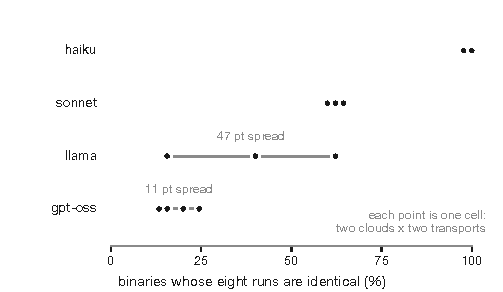
\includegraphics[width=0.78\textwidth]{fig2-determinismo.pdf}
\caption{Determinism at temperature $0.0$: the share of binaries whose eight runs return an
identical pass-rate, per model, with one point per cell. The spread within a model is the
distance between its clouds and transports --- the same nominal model is not equally stable
on different infrastructures.}
\label{fig:determinism}
\end{figure}

Second, \emph{the same nominal model is not equally stable on different clouds}, and on 45 binaries the
sampling supports that claim in exactly one of eight comparisons: llama on the native transport returns
identical scores on 24.4\% of binaries at one endpoint $[14.2, 38.7]$ and 66.7\% at the other $[52.1,
78.6]$, Wilson bands not touching. The other seven overlap and are not used as evidence. One clean case is
what these data support, on the same model and axis where T6 shows the largest endpoint effect in the
study, and the original collection isolates the same comparison.

\subsection{What the metric buys, measured}

Pass-rate has a floor reachable without reconstructing anything, and we measured it rather than
assuming it: the 53 runs that called \emph{no} tool average $0.1132$ against $0.6378$ for the 5{,}756
that called at least one. The floor exists and does not dominate --- the metric is a lower bound with a
measured floor, and the artifact carries the distribution.
\subsection{Declared covariates}

Two confounds were measured before the confirmatory numbers were read and neither is corrected for, since
correcting a pre-registered design after the fact is the freedom pre-registration exists to remove.
\emph{Calls per turn} is the one the ablation arm of \S\ref{sec:rq5} isolates, and it binds on two models
of four (\S\ref{sec:method}). \emph{Material acquired} is the second: replaying what each transport
actually requested, the native arm asks for more functions per binary in \emph{all eight} cells, most
strongly on llama at one endpoint ($-1.16$ functions, SD $0.90$), against six of eight originally. We do
not order that per-cell agreement against the size of the endpoint effect --- with four models the ordering
is indistinguishable from noise --- and the artifact carries both covariates in full.

\subsection{Scope}

The effect sizes are circumscribed twice over and both bounds are part of the result. They come from
\emph{one} family of tasks --- decompiled C binaries scored by unit tests --- on four models and two clouds,
so T3's $-9.83$pp is a measurement on this corpus rather than a quantity transferable elsewhere: a reader
who needs a number for their own setting should take the method and the variance decomposition, not the
point estimate. And every statement above concerns \emph{this} text protocol --- one call per turn, one line
of the response --- not textual tool calling in general, about which a leaderboard reporting both modes
finds the textual variant \emph{ahead} by 6pp on one model, against the direction that seeded this work.

\section{Discussion}
\label{sec:discussion}

\subsection{A null confirmatory result that is not a null finding}

Ten pre-registered tests, none surviving correction --- and the reason is measurable rather than
mysterious. The design was sized on a standard deviation borrowed from the preceding
chapter~\citep{companion2026baseline}, and that borrowing is where the study earns its keep: the
quantity borrowed turns out not to be a property of the model, so no care at design time would have
produced a different number of binaries. Where the pre-registration recorded 84\% run-to-run noise and
a floor of thirteen binaries, the same nominal contrast here gives 0.5\% and 668. Not an underestimate
--- an inversion, and the lever the previous chapter said would work is the one that buys nothing here.

This is the finding we did not go looking for, and \S\ref{sec:rq6} places it against the literature on
borrowed effect sizes. The consequence for a designer belongs here: inheriting that calibration would
not merely have left them under-powered, it would have sent their budget to the axis that buys
nothing. The rival account for the decomposition --- that
the granularity of the metric produces the spread on its own --- is bounded in
\S\ref{sec:granularita} by the two conditions it would and would not have to explain, with the
figures for each.

\subsection{Why the census carries the weight}

The confirmatory arm and the census differ in what it takes to overturn them. Every number in
\S\ref{sec:results} is a point estimate with an interval that a larger study could move; nothing in
\S\ref{sec:census} is an estimate, since an endpoint either returned that message or it did not and the
artifact carries the request that produced it. A referee who disbelieves the census can re-run the probe;
one who disbelieves the contrasts has to re-run 5{,}809 trials.


\subsection{When to discard a batch, and when not to}

Two batches were invalidated and re-collected rather than patched, and the rule separating them from the
one we kept is reusable. \textbf{Discard when the contaminating channel is systematic and asymmetric
between the compared arms; report and bound it otherwise.}

The larger invalidation --- 2{,}390 measurements --- meets that test exactly: the algorithm's name reached
the model through three separate channels and the two arms encountered one at different rates, so left in
place it would have turned part of the transport effect into a measure of how often each transport stumbled
onto the answer. No downstream analysis separates a contaminant that correlates with the
manipulated variable.

The shared working directory (\S\ref{sec:threats}) fails the same test in the other direction:
non-directional noise, some thirty times in the original batch's 5{,}805 measurements, with no asymmetry
between arms.
Discarding it would have been a gesture rather than a correction, so we bounded it, probed it, and
re-collected on isolated workspaces. Two practices made the rule applicable rather than rhetorical:
channels were enumerated per channel and not per intention --- the third was found because we listed every
place the model could read --- and both batches remain in the artifact with their recomputation.

\subsection{What an evaluation should report}

What follows amends an existing checklist rather than proposing a new one: the community guidelines already
require the harness to be described once it goes beyond bare API calls~\citep{baltes2026guidelines}, and each
field below either sharpens that requirement or extends it to one they do not name. Each costs a line in a
method section, and Table~\ref{tab:checklist} states them as fields because a recommendation phrased as prose
is one a reader agrees with and does not apply. The first carries the argument of \S\ref{sec:runtime}: a
model name does not identify a measurable system, the same nominal model on two clouds being two apparatuses
that differ in score stability as well as in score.

\begin{table}[t]
\centering
\caption{What an agentic evaluation should declare. The first four sharpen requirements that
already exist~\citep{baltes2026guidelines}; the last two have no counterpart in current
checklists.}
\label{tab:checklist}
\footnotesize
\setlength{\tabcolsep}{4pt}
\begin{tabular}{@{}p{0.26\linewidth}p{0.66\linewidth}@{}}
\toprule
field & what it means \\
\midrule
transport & how a tool call is encoded: native function calling, a textual protocol, typed
  code stubs --- and whether more than one call per turn is admitted \\
endpoint & which service served the weights, not only the model name \\
model and version & the identifier the endpoint accepts, including any regional prefix \\
configuration & temperature, token limits, turn budget, seed where honoured \\
\textbf{models excluded} & which models were considered and not measured \\
\textbf{reason for each} & the endpoint's own message, verbatim, or the policy that applied \\
\bottomrule
\end{tabular}
\end{table}

\subsection{Five propositions that should outlive this task}
\label{sec:proposizioni}

The effect sizes here belong to one task family, four models and two clouds, and we claim nothing beyond
that. What we offer beyond it are five propositions about how experiments of this kind behave, each
instantiated by this study rather than proved in general.

\begin{enumerate}
  \item The transport belongs beside temperature in a method section.
  \item An endpoint can produce missing experimental units, whose cost \S\ref{sec:bound} bounds.
  \item Variance components can be apparatus-specific, so an inherited calibration must be recomputed on
        one's own data as soon as the first cell exists.
  \item A pre-flight must exercise realistic conversational states: two of our eight mechanisms fire only
        in a state a single-call probe never reaches.
  \item Metric granularity limits what a variance decomposition can say. We report the floor and ceiling
        shares beside ours, and did not size the tests per task.
\end{enumerate}

\noindent
The artifact carries each with its argument.



\section{Threats to Validity}
\label{sec:threats}

Each threat is reported in the same four parts: what it is, how large it is, the diagnostic or
mitigation that answers it, and the residual.

\subsection{Construct validity: what pass-rate measures}

\textbf{Threat.} Pass-rate is a lower bound on semantic equivalence, and it has a floor: a
candidate written without consulting the decompiled program can still pass some tests, so part
of any score may be pattern-matching rather than reconstruction.

\textbf{Quantification.} The floor is measurable inside the study rather than assumed, and
\S\ref{sec:results} reports it: the runs that called no tool at all average 0.113 against 0.638 for those
that called at least one.

\textbf{Residual.} The floor exists and does not dominate, and both halves carry a number. Pass-rate is
reported as a lower bound throughout, and no claim in this paper requires it to be more.

\subsection{Construct validity: what a transport carries}

\textbf{Threat.} The transport contrast is a change of \emph{format} and also a change in the volume of
context the request carries. \S\ref{sec:runtime} reports the same quantity between two services; it also
differs between the two transports, on the axis this study exists to isolate.

\textbf{Quantification.} Median provider-reported input tokens per run, native over textual, across the
eight cells where both arms exist: $2.89$ and $2.47$ on gpt-oss (Databricks, Bedrock), $2.34$ and $1.02$ on
llama, $1.38$ and $1.37$ on haiku, and $0.75$ and $0.73$ on sonnet. The native arm is reported higher in six
cells of eight and lower in two, so the divergence has no fixed direction. T1 is the cell where this matters
most: gpt-oss issues exactly one call per turn, so it is the contrast with no batching confound to absorb
the difference.

\textbf{Diagnostic.} This is a component of the transport as evaluated, not a leak into it. Under native
calling the tool schemas travel in a \texttt{tools} field and results return in the provider's tool role;
under our prompted-text protocol both travel as ordinary messages. \textbf{The two implementations we
evaluated do not isolate serialisation format from context volume}, and the ablation arm of
\S\ref{sec:rq5} separates batching from format but not format from volume. Whether some other pairing of
implementations could hold context volume fixed while changing the encoding is a question this design does
not answer and does not foreclose.

\textbf{Residual.} The transport effects of \S\ref{sec:results} are therefore effects of a transport as
deployed rather than of a serialisation syntax holding all else equal, and a reader sizing their own study
should read them that way.

\subsection{Construct validity: what the ablation arm separates}

\textbf{Threat.} The constrained-native arm of \S\ref{sec:rq5} separates call batching from call format
only up to the two effects below.

\textbf{Quantification.} The constraint does not remove batching alone: forcing one call per turn also
changes the shape of the trajectory the model plans, so what the arm bounds is an upper limit on the
batching contribution rather than an estimate of it. And it covers one infrastructure and the two models
that batch at all --- on the other two the rate is exactly 1.000 calls per turn, so there is nothing to
remove and no contrast to run.

\textbf{Residual.} The arm therefore supports a ceiling rather than a point estimate --- at most 26\% and
13\% of the transport effect on the two models that batch (\S\ref{sec:rq5}) --- and the artifact carries
both bounds with the per-model rates.

\subsection{Internal validity: a working directory shared across cells}

\textbf{Threat.} Candidates were compiled in a directory keyed on the program and the run index and
nothing else, so under concurrent collection two cells could share a compilation path and a run compiling
another cell's candidate would be scored normally with no flag raised. The key omits the cell, so no
contrast is structurally exempt.

\textbf{Quantification.} The precondition --- two cells sharing a compilation path at the same moment ---
arose \textbf{thirty} times in the original batch of 5{,}805 measurements. The deposit carries the
mechanism, the write-to-read window and the probe these data admit.

\textbf{Mitigation.} The working directory now carries the cell, and the whole design was collected again
on workspaces isolated per cell. \textbf{That is what makes the re-collection the primary basis: the
mechanism is absent there by construction, not observed absent} --- thirty occurrences originally, zero
under 451 concurrent measurements that would have exposed it. This is a property of the code rather than
of either batch's numbers.

\textbf{Concordance with the original collection.} Four diagnostics were specified for the comparison,
and all four are met: six of eight contrasts keep their sign against a threshold of six; no test passes
its Holm threshold in either batch; seven of eight re-collected effects fall inside the original 95\%
interval, the exception being T7, whose original interval spans 0.3pp because that cell is almost
noiseless; and the noise share that inverted the sample-size calibration reproduces within an order of
magnitude, 0.1\%/$K_\infty{=}705$ against 0.5\%/668. Appendix~\ref{sec:appendice-provenienza} states when
each threshold was written and against what was known.

% Generata da analysis/tabella_riraccolta.py — non modificare a mano.
\begin{table}[t]
\centering
\caption{The same eight contrasts measured twice: the original collection, and an independent re-collection on workspaces isolated per cell. Differences in percentage points; the last column states whether the re-collected effect falls inside the original 95\% interval. The criteria and their thresholds were written before the comparison could be computed; their timing is stated precisely in \S\ref{sec:threats}, where it is weaker than the pre-registration's.}
\label{tab:riraccolta}
\footnotesize
\setlength{\tabcolsep}{5pt}
\begin{tabular}{@{}llrrc@{}}
\toprule
 & model & orig. & re-coll. & in CI \\
\midrule
T1 & gpt-oss-120b & $-6.4$ & $-6.6$ & yes \\
T2 & llama-3.3-70b & $+3.5$ & $+2.2$ & yes \\
T3 & claude-haiku-4-5 & $-10.4$ & $-9.8$ & yes \\
T4 & claude-sonnet-4-5 & $+2.1$ & $-1.0$ & yes \\
T5 & gpt-oss-120b & $+3.4$ & $+3.3$ & yes \\
T6 & llama-3.3-70b & $-8.9$ & $-7.9$ & yes \\
T7 & claude-haiku-4-5 & $-0.1$ & $+0.2$ & no \\
T8 & claude-sonnet-4-5 & $-0.7$ & $-0.9$ & yes \\
\bottomrule
\end{tabular}
\end{table}

% criterio 1, segni concordi: 6/8 (soglia 6) -> invariato
% criterio 3, copertura IC95: 7/8 (soglia 6) -> invariato


\textbf{Residual.} The original batch is reported in full beside the primary one rather than invalidated:
the criterion this programme applies to invalidation is a systematic, arm-asymmetric channel
(\S\ref{sec:discussion}), and the shared workspace is neither.

\subsection{Conclusion validity: the guards, and their perimeter}

\textbf{Threat and residual.} The analysis is protected by a content-hash chain over six named files ---
the pre-registration, the frozen analysis and power scripts, the held-out corpus, the collector, and the
comparison script --- and by an append-only convention on the result directory whose guarantee is the
committed history. Both perimeters are stated so that a claim of precedence can be checked against the
right one, and the artifact enumerates them.

\subsection{Conclusion validity: the estimator}

\textbf{Threat.} The pre-registered test is a paired $t$ over per-binary means, which discards the
within-binary structure a run-level model would use.

\textbf{Quantification.} What we can measure is where the variance sits, and Table~\ref{tab:variance}
measures it: on T3 and T6, the two contrasts on which the variance decomposition is most informative,
run-to-run noise is 0.5\% and 9.1\% of the
paired variance, so almost all of it is between binaries rather than within them. On T5 it is 93\%, and on
T7 and T8 the estimator does not fit at all.

\textbf{Diagnostic.} The run-level counterfactual is computed in Appendix~\ref{sec:appendice-glmm} and
agrees: a marginal model with cluster-robust errors reproduces the frozen test's reading on all three
contrasts it covers, and none passes Holm.

\textbf{Residual.} That model is reported as a sensitivity analysis rather than substituted for the frozen
estimator: choosing an estimator after seeing which contrasts it favours is the freedom the freeze exists
to remove.

\subsection{External validity: what the design does not settle}

\textbf{Threat.} The design manipulates transport and infrastructure at a fixed \emph{nominal model
identity}, and the weaker phrase is deliberate: the design does not verify that a nominally identical
model is byte-identical across two providers, and neither provider exposes enough to settle it.

\textbf{Quantification.} The divergence matters rather than being hypothetical: on the one axis where the
Wilson bands separate, the same nominal model returns identical scores on 24.4\% of binaries at one cloud
against 66.7\% at the other (\S\ref{sec:results}).

\textbf{Residual.} The rates are reported at the level the design identifies --- the deployed service ---
since attributing them further would require knowing what each provider serves. The scope of every effect
size reported here is one task family, four models and two clouds, as the pre-registration bounds it.

\section{Conclusion}
\label{sec:conclusion}

Four models, two managed clouds and two tool transports were run against a pre-registration and an
analysis script frozen together before any row existed, save two tests documented in
\S\ref{sec:method}. The confirmatory result comes from the independent re-collection on workspaces
isolated per cell --- 5{,}809 measured trials --- designated the primary basis in writing before it
produced a row; the original batch of 5{,}805 sits beside it as a replication, and the two agree on all
four criteria frozen in advance. None of the ten pre-registered tests survives Holm correction, and the
three contrasts reaching nominal significance are the three least powered in the study --- reported
together with the achieved power, since power determines what a $p$-value can mean.

The design was mis-sized, and the reason is itself the finding: the calibration inherited from the
preceding chapter did not misjudge a magnitude, it inverted which lever binds. Where that chapter found
84\% run-to-run noise and a floor of thirteen binaries, the same nominal contrast gives 0.5\% and 668. A
calibration is a claim about an apparatus, and it does not travel.

What does not depend on a $p$-value is the census: six pre-collection mechanisms remove a model from an
evaluation, each with the endpoint's own words, plus two conversational-state failures that appeared only
while collecting. The split is the practical finding --- a pre-flight probe reaches the first six and
\emph{cannot} reach the last two, so a harness certified healthy can still lose a cell after the money is
spent, and existing taxonomies of serving failures begin one step later.

Two properties of the apparatus usually assumed turned out to be measurable and to vary. Temperature
zero is not determinism: one model returns identical runs on 91--100\% of binaries and another on
20--24\%. And in the one comparison of eight where the sampling bands separate, the same nominal model
returns identical scores on 24.4\% of tasks at one endpoint and 66.7\% at the other, which makes score
stability a property of the serving stack rather than of a decoding parameter.

The transport moves a number, and that is a bias: bounded, correctable, already visible in a public leaderboard. The endpoint deletes a row, and that is a selection: the model it refused has no line
to correct. Evaluations report the first inconsistently and the second not at all. Declaring the
transport, the endpoint, and the models each endpoint refused costs three lines in a method section, and
without them a published agentic number does not identify the system it describes.

% sections/10-artifact: assorbita nelle Declarations il 2026-08-16.
% Ripeteva parola per parola append-only, documenti di successione e catena
% degli hash, che EMSE vuole sotto «Statements and Declarations». Il raddoppio
% faceva sembrare il paper occupato dalla propria igiene piu' che dai risultati.
% IL TITOLO E L'ORDINE VENGONO DALLA LETTERA DI RITORNO, non dalle istruzioni per autori.
% La prima sottomissione (EMSE-D-26-00987) e' stata restituita per completezza: le istruzioni
% pubbliche dicono «Statements and Declarations», l'ufficio editoriale chiede «Declarations» con
% sei sottosezioni nominate e in quest'ordine. Dove le due fonti divergono vince la lettera, che
% e' la piu' specifica e la piu' recente. Nessuna di queste sei si omette: se una non si applica
% si scrive che non si applica, ed e' esattamente cio' che la lettera prescrive.
\section*{Declarations}

\subsection*{Funding}

This work received no specific grant from any funding agency. Inference costs were borne by the
author's institution and are itemised per arm in the replication package, so the cost of each
number is auditable beside the number.

There are no acknowledgements: the author is the sole contributor, and this statement is therefore
already separate from any.

\subsection*{Ethical approval}

Not applicable. The study involves no human participants and no personal data. It measures
commercial inference endpoints under their ordinary terms of use, at a request rate below the
published limits of both platforms, and reports the responses those endpoints returned.

\subsection*{Informed consent}

Not applicable. The study has no human participants, so there is no one from whom consent could
be sought. The subjects of measurement are four commercial inference endpoints, and what was
collected from them is the text they returned to documented requests.

\subsection*{Author contributions}

<autore> is the sole author and carried out the whole of the work: conceptualisation,
the pre-registration and its frozen analysis plan, the harness for both transports, data
collection across both clouds, the analysis scripts, the interpretation, and the writing of the
manuscript. There are no other authors.

\subsection*{Data availability statement}

\label{sec:artifact}

The replication package contains the 45 stripped binaries and their test suites, the decompilations, the
harness with both transports, every raw result row including the two invalidated batches, the per-turn
session traces, the frozen pre-registration and analysis script with their content hashes, and the dated
succession documents accounting for every change to a frozen file. Each number in this paper is produced
by a script released with it, re-running from the released rows; no figure is drawn by hand.

% Il repository e' il deposito operativo, citato per URL; il DOI permanente si deposita
% all'accettazione, perche' un DOI si ottiene depositando e non prima. La frase sotto dice
% quello che e' vero oggi invece di promettere un identificatore che non esiste ancora.
The two numbers this paper takes from the preceding chapter are re-runnable here: the deposit carries a
snapshot of exactly the cells they need with their per-turn logs, so both the calibration inversion and the
tool-exposure asymmetry recompute without leaving the artifact. It does not carry the rest of that chapter,
and says so.

Three commands regenerate everything a reader might want to check, and they are the ones we ran:

\begin{quote}\footnotesize\ttfamily\raggedright
python3 analysis/numeri\_paper.py \textrm{--- every number in prose}\\
python3 analysis/tabella\_principale.py \textrm{--- Table \ref{tab:tests}}\\
python3 analysis/tabella\_principale.py -{}-varianza \textrm{--- Table \ref{tab:variance}}
\end{quote}

\noindent
The first carries its own known-answer check: pointed at the original collection it must reproduce the
numbers this paper reported before the re-collection, and exits non-zero otherwise --- which is what
makes the new series trustworthy rather than merely recomputed, and what caught a ratio reported as 77
whose value is 76.3. Each collection is selected by the same three environment variables
(\texttt{C2\_RESULTS}, \texttt{C2\_PATTERN}, \texttt{C2\_PREFISSO}); setting only one yields an index
built on one batch and queried with the keys of the other, which returns zero rather than raising.

The package is openly available at \artifacturl{}\ and will be deposited on a permanent archive with a
DOI on acceptance. Cloud workspace and profile names, absolute paths and one internal account identifier
are replaced by placeholders, because infrastructure names belong to an employer rather than to a study,
and \texttt{REDAZIONE.md} lists every substitution; nothing else is redacted, the venue being
single-blind. Redaction changes the content hash of a frozen file and this paper quotes those hashes, so
the deposit carries its own recomputed table alongside that document, with the integrity guard run inside
the deposit and passing there. Two further properties are checkable rather than asserted: the result
directory is append-only, invalidated batches moved and annotated with the recomputation beside each
rather than deleted; and every change to a frozen file carries a document written before the change,
declaring the previous and the new hash, with a guard rejecting any divergence no document accounts
for.

\subsection*{Conflict of interest}

The author declares no competing interests. The two serving platforms measured in this study
were selected because the institution already held accounts on both; neither vendor was
contacted, informed, or involved at any stage, and neither reviewed this manuscript.

\subsection*{Reporting checklist}

The study follows the community guidelines for empirical studies involving language
models~\citep{baltes2026guidelines}: model identifiers, versions and configuration are reported
per cell (\S\ref{sec:method}); the system and harness design is described and released; per-turn
session traces are published for every run rather than summarised; and two of the four models
under evaluation are open-weight, so that their scores can be independently re-run on
infrastructure the reader controls. The guidelines' requirement that we sharpen --- reporting
the transport --- is the subject of the paper rather than only its practice.

\subsection*{Use of language models in this work}

Language models are the object of study here, and they were also used as a tool while
conducting it --- to draft and review code and prose --- which the community guidelines ask to
be declared separately from their role as
subject~\citep{baltes2026guidelines}. No measurement, no number, and no decision reported in
this paper was produced by that use: every quantity comes from a committed script run against
committed rows, and the guards described above exist precisely because an author who accepts a
generated number without recomputing it has no way to notice when it is wrong.


% Il \nocite{*} e' stato tolto il 2026-08-15: le sezioni citano davvero, e la verifica dice
% La verifica si rifa' a ogni compilazione: e' uno script, non questo commento,
% a dire quante chiavi sono citate e quante definite.
% Nota storica di quando serviva: uno
% scheletro senza una sola \cite produce una bibliografia vuota, che non compila: senza
% questa riga non potrei dire "lo scheletro compila", potrei solo scriverlo.
% Lasciarlo nel paper finito elencherebbe opere mai citate.
% R8 — sensibilita' NON pre-registrata. Sta in appendice e non nei risultati per una ragione
% precisa: il paper si regge sulla distinzione fra cio' che era congelato e cio' che non lo era,
% e mettere un test aggiunto dopo accanto a quelli pre-registrati la cancellerebbe.
\appendix
\section{Distribution-free sensitivity for the pre-registered family}
\label{sec:appendice-permutazione}

The pre-registered test is a paired $t$ over 45 binaries, which assumes approximately normal paired
differences. On this metric they are not: pass-rate over five unit tests takes six values, 53\% of rows
sit at an extreme, and the paired difference of two such means is discrete with short tails. If a test
assuming no distribution reaches the same conclusion, the assumption was not carrying the result. For
paired differences the exact permutation test is the sign flip --- under the null the sign of each
binary's difference is exchangeable --- and with $2^{45}$ assignments we sample 50{,}000 at a declared
seed and report the Monte Carlo error of the $p$ itself, a sampled $p$ being an estimate.

\begin{table}[h]
\centering
\caption{Sign-flip permutation against the pre-registered Student's $t$. Holm applies the same
fixed $m=10$ as the pre-registered family.}
\label{tab:permutazione}
\footnotesize
\setlength{\tabcolsep}{4pt}
\begin{tabular}{@{}lrrrr@{}}
\toprule
& $p$ Student & $p$ permutation & MC error & difference \\
\midrule
T6 & 0.0191 & 0.0135 & 0.0008 & $-0.0055$ \\
T3 & 0.0218 & 0.0228 & 0.0011 & $+0.0010$ \\
T1 & 0.0334 & 0.0319 & 0.0012 & $-0.0014$ \\
T2 & 0.1107 & 0.1194 & 0.0023 & $+0.0087$ \\
T5 & 0.1159 & 0.1205 & 0.0023 & $+0.0046$ \\
T8 & 0.2844 & 0.3267 & 0.0033 & $+0.0423$ \\
T7 & 0.2095 & 0.5032 & 0.0035 & $+0.2937$ \\
T4 & 0.6363 & 0.7754 & 0.0030 & $+0.1391$ \\
\bottomrule
\end{tabular}
\end{table}

\textbf{No test passes Holm under either series}, so the family outcome does not depend on the
distributional assumption and the objection closes without altering anything pre-registered.

Two contrasts disagree by more than the Monte Carlo error, informatively: T7 moves from 0.21 to 0.50 and
T4 from 0.64 to 0.78, and both are the contrasts with the smallest observed variance, where the $t$
divides by a standard error the permutation test never uses. That the $t$ reports smaller $p$ exactly
where variance is smallest is the mechanism rather than a coincidence, and it supports the reading of
\S\ref{sec:results}: T7's narrow interval reflects absence of noise rather than power. This analysis is
not pre-registered and does not replace the frozen one --- had the two diverged on the family outcome the
reportable conclusion would still be the pre-registered one, with the divergence declared.


\bibliographystyle{plainnat}
\bibliography{references}

\end{document}
